\PassOptionsToPackage{unicode=true}{hyperref} % options for packages loaded elsewhere
\PassOptionsToPackage{hyphens}{url}
\documentclass[12pt,ignorenonframetext,]{beamer}
\IfFileExists{pgfpages.sty}{\usepackage{pgfpages}}{}
\setbeamertemplate{caption}[numbered]
\setbeamertemplate{caption label separator}{: }
\setbeamercolor{caption name}{fg=normal text.fg}
\beamertemplatenavigationsymbolsempty
\setbeameroption{show notes}
\usepackage{lmodern}
\usepackage{amssymb,amsmath}
\usepackage{ifxetex,ifluatex}
\usepackage{fixltx2e} % provides \textsubscript
\ifnum 0\ifxetex 1\fi\ifluatex 1\fi=0 % if pdftex
  \usepackage[T1]{fontenc}
  \usepackage[utf8]{inputenc}
\else % if luatex or xelatex
  \ifxetex
    \usepackage{mathspec}
  \else
    \usepackage{fontspec}
\fi
\defaultfontfeatures{Ligatures=TeX,Scale=MatchLowercase}







\fi

  \usetheme[]{metropolis}






% use upquote if available, for straight quotes in verbatim environments
\IfFileExists{upquote.sty}{\usepackage{upquote}}{}
% use microtype if available
\IfFileExists{microtype.sty}{%
  \usepackage{microtype}
  \UseMicrotypeSet[protrusion]{basicmath} % disable protrusion for tt fonts
}{}


\newif\ifbibliography
  \usepackage[round]{natbib}
  \bibliographystyle{abbrvnat}


\hypersetup{
      pdftitle={Machine Learning in R},
        pdfauthor={Kasun Bandara},
          pdfborder={0 0 0},
    breaklinks=true}
%\urlstyle{same}  % Use monospace font for urls




  \usepackage{color}
  \usepackage{fancyvrb}
  \newcommand{\VerbBar}{|}
  \newcommand{\VERB}{\Verb[commandchars=\\\{\}]}
  \DefineVerbatimEnvironment{Highlighting}{Verbatim}{commandchars=\\\{\}}
  % Add ',fontsize=\small' for more characters per line
  \usepackage{framed}
  \definecolor{shadecolor}{RGB}{248,248,248}
  \newenvironment{Shaded}{\begin{snugshade}}{\end{snugshade}}
  \newcommand{\AlertTok}[1]{\textcolor[rgb]{0.94,0.16,0.16}{#1}}
  \newcommand{\AnnotationTok}[1]{\textcolor[rgb]{0.56,0.35,0.01}{\textbf{\textit{#1}}}}
  \newcommand{\AttributeTok}[1]{\textcolor[rgb]{0.77,0.63,0.00}{#1}}
  \newcommand{\BaseNTok}[1]{\textcolor[rgb]{0.00,0.00,0.81}{#1}}
  \newcommand{\BuiltInTok}[1]{#1}
  \newcommand{\CharTok}[1]{\textcolor[rgb]{0.31,0.60,0.02}{#1}}
  \newcommand{\CommentTok}[1]{\textcolor[rgb]{0.56,0.35,0.01}{\textit{#1}}}
  \newcommand{\CommentVarTok}[1]{\textcolor[rgb]{0.56,0.35,0.01}{\textbf{\textit{#1}}}}
  \newcommand{\ConstantTok}[1]{\textcolor[rgb]{0.00,0.00,0.00}{#1}}
  \newcommand{\ControlFlowTok}[1]{\textcolor[rgb]{0.13,0.29,0.53}{\textbf{#1}}}
  \newcommand{\DataTypeTok}[1]{\textcolor[rgb]{0.13,0.29,0.53}{#1}}
  \newcommand{\DecValTok}[1]{\textcolor[rgb]{0.00,0.00,0.81}{#1}}
  \newcommand{\DocumentationTok}[1]{\textcolor[rgb]{0.56,0.35,0.01}{\textbf{\textit{#1}}}}
  \newcommand{\ErrorTok}[1]{\textcolor[rgb]{0.64,0.00,0.00}{\textbf{#1}}}
  \newcommand{\ExtensionTok}[1]{#1}
  \newcommand{\FloatTok}[1]{\textcolor[rgb]{0.00,0.00,0.81}{#1}}
  \newcommand{\FunctionTok}[1]{\textcolor[rgb]{0.00,0.00,0.00}{#1}}
  \newcommand{\ImportTok}[1]{#1}
  \newcommand{\InformationTok}[1]{\textcolor[rgb]{0.56,0.35,0.01}{\textbf{\textit{#1}}}}
  \newcommand{\KeywordTok}[1]{\textcolor[rgb]{0.13,0.29,0.53}{\textbf{#1}}}
  \newcommand{\NormalTok}[1]{#1}
  \newcommand{\OperatorTok}[1]{\textcolor[rgb]{0.81,0.36,0.00}{\textbf{#1}}}
  \newcommand{\OtherTok}[1]{\textcolor[rgb]{0.56,0.35,0.01}{#1}}
  \newcommand{\PreprocessorTok}[1]{\textcolor[rgb]{0.56,0.35,0.01}{\textit{#1}}}
  \newcommand{\RegionMarkerTok}[1]{#1}
  \newcommand{\SpecialCharTok}[1]{\textcolor[rgb]{0.00,0.00,0.00}{#1}}
  \newcommand{\SpecialStringTok}[1]{\textcolor[rgb]{0.31,0.60,0.02}{#1}}
  \newcommand{\StringTok}[1]{\textcolor[rgb]{0.31,0.60,0.02}{#1}}
  \newcommand{\VariableTok}[1]{\textcolor[rgb]{0.00,0.00,0.00}{#1}}
  \newcommand{\VerbatimStringTok}[1]{\textcolor[rgb]{0.31,0.60,0.02}{#1}}
  \newcommand{\WarningTok}[1]{\textcolor[rgb]{0.56,0.35,0.01}{\textbf{\textit{#1}}}}



% Prevent slide breaks in the middle of a paragraph:
\widowpenalties 1 10000
\raggedbottom

  \AtBeginPart{
    \let\insertpartnumber\relax
    \let\partname\relax
    \frame{\partpage}
  }
  \AtBeginSection{
    \ifbibliography
    \else
      \let\insertsectionnumber\relax
      \let\sectionname\relax
      \frame{\sectionpage}
    \fi
  }
  \AtBeginSubsection{
    \let\insertsubsectionnumber\relax
    \let\subsectionname\relax
    \frame{\subsectionpage}
  }



\setlength{\parindent}{0pt}
\setlength{\parskip}{6pt plus 2pt minus 1pt}
\setlength{\emergencystretch}{3em}  % prevent overfull lines
\providecommand{\tightlist}{%
  \setlength{\itemsep}{0pt}\setlength{\parskip}{0pt}}

  \setcounter{secnumdepth}{0}


  \usepackage{subfig}

  \title[]{Machine Learning in R}

  \subtitle{R-Ladies Colombo Chapter}

  \author[
        Kasun Bandara
    ]{Kasun Bandara}

  \institute[
    ]{
    Melbourne Centre for Data Science, University of Melbourne, Australia.
    }

\date[
      29 March, 2021
  ]{
      29 March, 2021
        }


\begin{document}

% Hide progress bar and footline on titlepage
  \begin{frame}[plain]
  \titlepage
  \end{frame}



\begin{frame}

\begin{figure}

\includegraphics[scale=0.22]{images/kasun}
\end{figure}

\end{frame}

\hypertarget{introduction}{%
\section{Introduction}\label{introduction}}

\begin{frame}{About me}
\protect\hypertarget{about-me}{}

\begin{itemize}
\tightlist
\item
  2015 Graduated in Computer Science from University of Colombo School
  of Computing
\item
  2015 Joined WSO2 Inc.~as a Software Engineer
\item
  2016-2020 Ph.D.~in Computer Science, Monash University, Australia

  \begin{itemize}
  \tightlist
  \item
    Topic: Forecasting In Big Data With Recurrent Neural Networks
  \item
    Machine Learning for Time Series Forecasting
  \item
    Research Internship at Walmart Labs, San Francisco, USA
  \item
    Research Scientist at Turning Point, Melbourne, Australia
  \item
    Data Science Tutor, Faculty of IT, Monash University
  \end{itemize}
\item
  2021 Research Fellow, University of Melbourne
\end{itemize}

\end{frame}

\begin{frame}{About me (2)}
\protect\hypertarget{about-me-2}{}

\begin{itemize}
\tightlist
\item
  Research Interests

  \begin{itemize}
  \tightlist
  \item
    Global Forecasting Models
  \item
    Hierarchical Forecasting
  \item
    Retail sales/demand forecasting
  \item
    Renewable energy production forecasting (solar)
  \end{itemize}
\item
  Competition Fanatic !

  \begin{itemize}
  \tightlist
  \item
    M5 Forecasting Competition (\textbf{Gold Medalist})
  \item
    IEEE CIS Energy Forecasting Competition (\textbf{4th Place})
  \item
    Air-Liquide Energy Forecasting Competition (\textbf{4th Place})
  \item
    ANZ Customer Segmentation Challenge (\textbf{Top Performer})
  \end{itemize}
\end{itemize}

\end{frame}

\begin{frame}{What is Data Science ?}
\protect\hypertarget{what-is-data-science}{}

Data Science is an interdisciplinary field that permits you to extract
information from organized or unstructured data.

\begin{figure}
  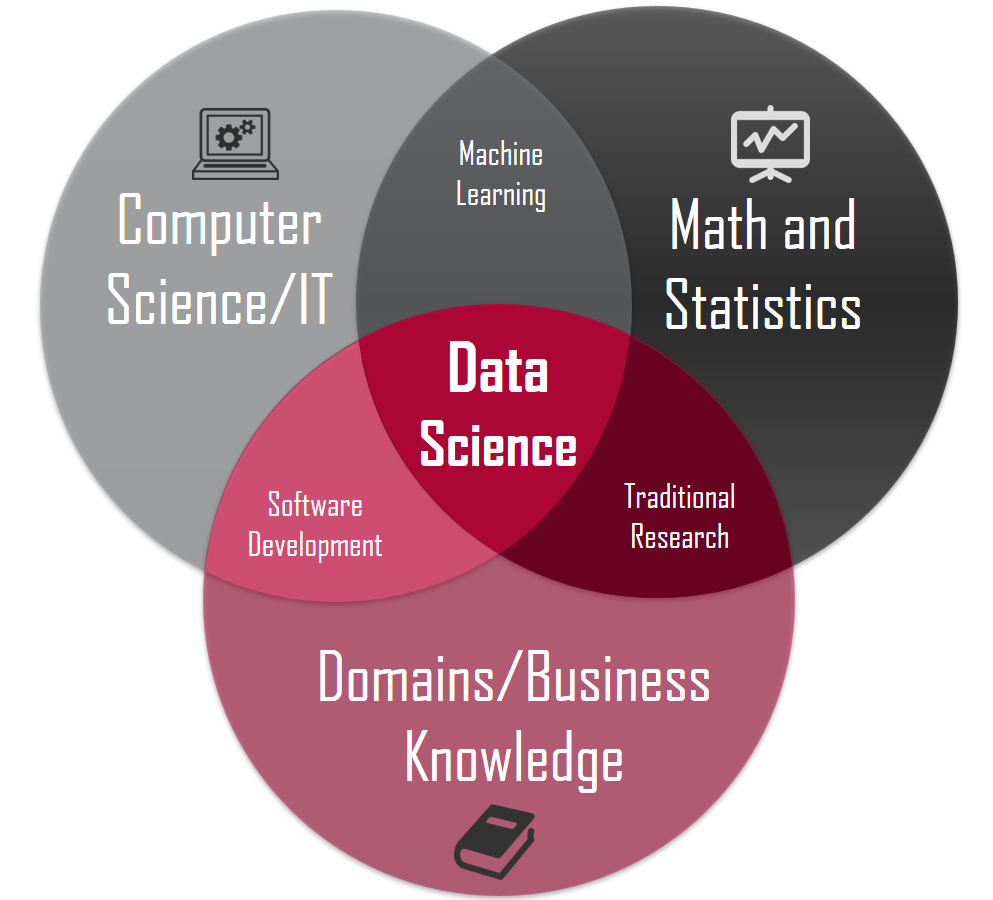
\includegraphics[width=.5\textwidth,height=.5\textheight,keepaspectratio]{images/datascience.jpeg}
  \caption{An intersection of many fields of science%
    \footnote{%
     \tiny{Image source: https://medium.com/believing-these-8-myths-about-what-is-data-science-keeps-you-from-growing-528f1bd240dc} 
    }%
  }
\end{figure}

\end{frame}

\begin{frame}{Data Science Life Cycle}
\protect\hypertarget{data-science-life-cycle}{}

Known as the O.S.E.M.N. framework.

\begin{figure}
  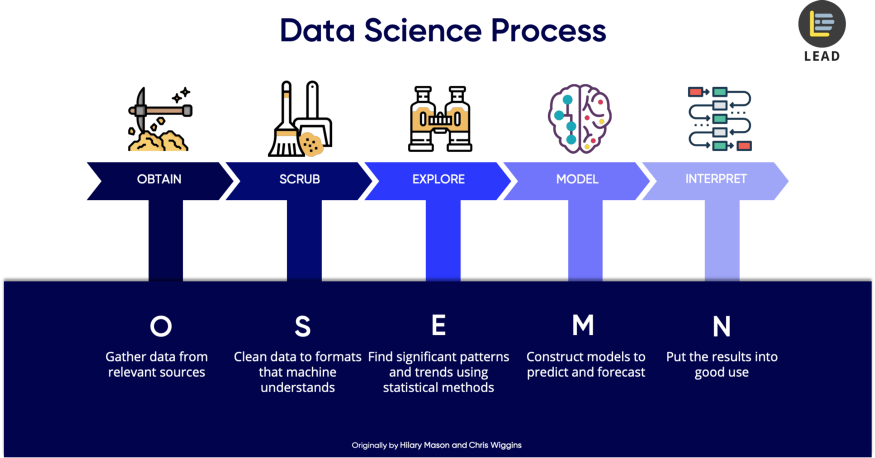
\includegraphics[width=.8\textwidth,height=.8\textheight,keepaspectratio]{images/osemn.png}
  \caption{Data Science Process%
    \footnote{%
     \tiny{Image source: https://towardsdatascience.com/5-steps-of-a-data-science-project-lifecycle-26c50372b492} 
    }%
  }
\end{figure}

\end{frame}

\begin{frame}{Obtain (O)}
\protect\hypertarget{obtain-o}{}

\begin{itemize}
\tightlist
\item
  Retrieving data from multiple sources of inputs.\\

  \begin{itemize}
      \item Structured Data: RDBMS, Tabular Data, CSV, TSV.
      \item Unstructured Data: NoSQL Databases, API Data (Twitter, Facebook).
  \end{itemize}
   \vspace{2mm}
\item
  Databases: \texttt{\{odbc\}} \vspace{2mm}
\item
  Scraping data from websites: \texttt{\{rvest\}} \vspace{2mm}
\item
  Data platforms: \textbf{Kaggle}, \textbf{UCI}, \textbf{Competition
  Datasets}, \textbf{Government APIs}
\end{itemize}

\end{frame}

\begin{frame}[fragile]{Example of \texttt{\{rvest\}}}
\protect\hypertarget{example-of}{}

\tiny

\begin{Shaded}
\begin{Highlighting}[]
\KeywordTok{library}\NormalTok{(rvest)}
\KeywordTok{library}\NormalTok{(dplyr)}
\KeywordTok{set.seed}\NormalTok{(}\DecValTok{1234}\NormalTok{)}

\CommentTok{# reading the HTML page (Lord of the Rings)}
\NormalTok{lor_movie <-}\StringTok{ }\KeywordTok{read_html}\NormalTok{(}\StringTok{"https://www.imdb.com/title/tt0120737/"}\NormalTok{)}

\CommentTok{# Scraping the movie rating.}
\NormalTok{lor_movie }\OperatorTok
\StringTok{  }\KeywordTok{html_node}\NormalTok{(}\StringTok{"strong span"}\NormalTok{) }\OperatorTok
\StringTok{  }\KeywordTok{html_text}\NormalTok{() }\OperatorTok
\StringTok{  }\KeywordTok{as.numeric}\NormalTok{()}
\CommentTok{#[1] 8.8}

\CommentTok{# Scraping the cast.}
\NormalTok{lor_movie }\OperatorTok
\StringTok{  }\KeywordTok{html_nodes}\NormalTok{(}\StringTok{"#titleCast .itemprop span"}\NormalTok{) }\OperatorTok
\StringTok{  }\KeywordTok{html_text}\NormalTok{()}

\CommentTok{# Scraping the movie poster.}
\NormalTok{lor_movie }\OperatorTok
\StringTok{  }\KeywordTok{html_nodes}\NormalTok{(}\StringTok{"#img_primary img"}\NormalTok{) }\OperatorTok
\StringTok{  }\KeywordTok{html_attr}\NormalTok{(}\StringTok{"src"}\NormalTok{)}
\end{Highlighting}
\end{Shaded}

\normalsize

\end{frame}

\begin{frame}{Scrub (S)}
\protect\hypertarget{scrub-s}{}

\begin{itemize}
\tightlist
\item
  Also known as \textbf{data pre-processing}, \textbf{data wrangling}.\\
  \vspace{2mm}
\item
  Converting the data into a unified, suitable format

  \begin{itemize}
      \item Easier for the data exploration process.
      \item What your predictive algorithm expects ?
      \item \textbf{tidyverse} \texttt{\{dplyr,tidyr,stringr,tibble,purr,ggplot2\}}
  \end{itemize}
   \vspace{2mm}
\item
  Handles data issues

  \begin{itemize}
      \item Cleaning: Missing values, Outliers, Noisy data.
      \item Transformation: Normalisation, Feature Discretization.
      \item Reduction: Feature selection, Dimensionality reduction.
  \end{itemize}
\end{itemize}

\end{frame}

\begin{frame}[fragile]{Missing Value Imputation}
\protect\hypertarget{missing-value-imputation}{}

\tiny

\begin{Shaded}
\begin{Highlighting}[]
\KeywordTok{library}\NormalTok{(simputation)}
\KeywordTok{set.seed}\NormalTok{(}\DecValTok{1234}\NormalTok{)}

\CommentTok{# Loading iris dataset and randomly inserting NAs.}
\NormalTok{df <-}\StringTok{ }\NormalTok{iris}
\NormalTok{df_NA <-}\StringTok{ }\KeywordTok{as.data.frame}\NormalTok{(}\KeywordTok{lapply}\NormalTok{(df, }\ControlFlowTok{function}\NormalTok{(imp) imp[ }\KeywordTok{sample}\NormalTok{(}\KeywordTok{c}\NormalTok{(}\OtherTok{TRUE}\NormalTok{, }\OtherTok{NA}\NormalTok{), }
        \DataTypeTok{prob =} \KeywordTok{c}\NormalTok{(}\FloatTok{0.85}\NormalTok{, }\FloatTok{0.15}\NormalTok{), }\DataTypeTok{size =} \KeywordTok{length}\NormalTok{(imp), }\DataTypeTok{replace =} \OtherTok{TRUE}\NormalTok{)]))}

\CommentTok{# Using median to impute the missing values.}
\NormalTok{median_imputed <-}\StringTok{ }\KeywordTok{impute_median}\NormalTok{(df_NA, }
\NormalTok{                                Sepal.Length }\OperatorTok{~}\StringTok{ }\NormalTok{Species)}

\CommentTok{# Using linear regression to impute the missing values.}
\NormalTok{linear_imputed <-}\StringTok{ }\KeywordTok{impute_lm}\NormalTok{(df_NA, Sepal.Length }\OperatorTok{~}\StringTok{ }\NormalTok{Sepal.Width }\OperatorTok{+}\StringTok{ }\NormalTok{Species)}

\CommentTok{# Using CART algorithm to impute the missing values.}
\NormalTok{cart_imputed <-}\StringTok{ }\KeywordTok{impute_cart}\NormalTok{(df_NA, Species }\OperatorTok{~}\StringTok{ }\NormalTok{.)}

\CommentTok{# Imputing multiple variables at once.}
\NormalTok{multivariable_imputed <-}\StringTok{ }\KeywordTok{impute_rlm}\NormalTok{(df_NA, Sepal.Length }\OperatorTok{+}\StringTok{ }\NormalTok{Sepal.Width }
                                    \OperatorTok{~}\StringTok{ }\NormalTok{Petal.Length }\OperatorTok{+}\StringTok{ }\NormalTok{Species)}

\CommentTok{# Imputing using a pre-trained model.}
\NormalTok{model <-}\StringTok{ }\KeywordTok{lm}\NormalTok{(Sepal.Length }\OperatorTok{~}\StringTok{ }\NormalTok{Sepal.Width }\OperatorTok{+}\StringTok{ }\NormalTok{Species, }\DataTypeTok{data=}\NormalTok{iris)}
\NormalTok{model_imputed <-}\StringTok{ }\KeywordTok{impute}\NormalTok{(df_NA, Sepal.Length }\OperatorTok{~}\StringTok{ }\NormalTok{model)}
\end{Highlighting}
\end{Shaded}

\normalsize

\end{frame}

\begin{frame}{Dealing with Outliers}
\protect\hypertarget{dealing-with-outliers}{}

\begin{itemize}
\tightlist
\item
  A data point that differs significantly from other observations.\\
  \vspace{2mm}
\item
  Observations that distort your analysis.

  \begin{itemize}
      \item Boxplot visualisation: \texttt{\{ggplot2\}}
      \item Grubbs’s test, Dixon’s test, Rosner’s test: \texttt{\{outliers\}}
      \item Outlier detection algorithms: \texttt{\{OutlierDetection\}}
      \item \textbf{outlierTest()} from \texttt{\{car\}}
      \item \textbf{lofactor()} from \texttt{\{DMwR\}} (Local Outlier Factor)
  \end{itemize}
   \vspace{2mm}
\item
  Anomaly detection is itself a different research area !

  \begin{itemize}
      \item One Class SVM, IsolationForest
      \item Unsupervised algorithms (Clustering)
      \item Time series: \texttt{\{tsoutliers,oddstream,stray\}}
  \end{itemize}
\end{itemize}

\end{frame}

\begin{frame}{Feature Selection}
\protect\hypertarget{feature-selection}{}

\begin{itemize}
\tightlist
\item
  Removing redundant features from the dataset. \vspace{2mm}
\item
  Computational complexity, Address model overfitting. \vspace{2mm}
\item
  \textbf{Filter Methods}

  \begin{itemize}
      \item Features are selected based on a statistical score.
      \item Independent of any machine learning algorithm.
      \item \textbf{Pearson’s Correlation, Chi-Square, PCA}
  \end{itemize}
   \vspace{2mm}
\item
  \textbf{Wrapper Methods}

  \begin{itemize}
      \item A subset of features are used to train a model.
      \item Forward, Backward, Recursive elimination.
      \item Inbuilt penalization functions: \textbf{LASSO, RIDGE} regression 
      \item \texttt{\{Boruta,caret,glmnet\}}
  \end{itemize}
\end{itemize}

\end{frame}

\begin{frame}[fragile]{Using Correlation}
\protect\hypertarget{using-correlation}{}

\tiny

\begin{Shaded}
\begin{Highlighting}[]
\KeywordTok{library}\NormalTok{(GGally)}
\KeywordTok{library}\NormalTok{(dplyr)}
\KeywordTok{set.seed}\NormalTok{(}\DecValTok{1234}\NormalTok{)}

\CommentTok{# Plotting the feature correlations.}
\NormalTok{iris }\OperatorTok\StringTok{ }\KeywordTok{select}\NormalTok{(}\OperatorTok{-}\NormalTok{Species) }\OperatorTok\StringTok{ }\KeywordTok{ggpairs}\NormalTok{()}
\end{Highlighting}
\end{Shaded}

\begin{center}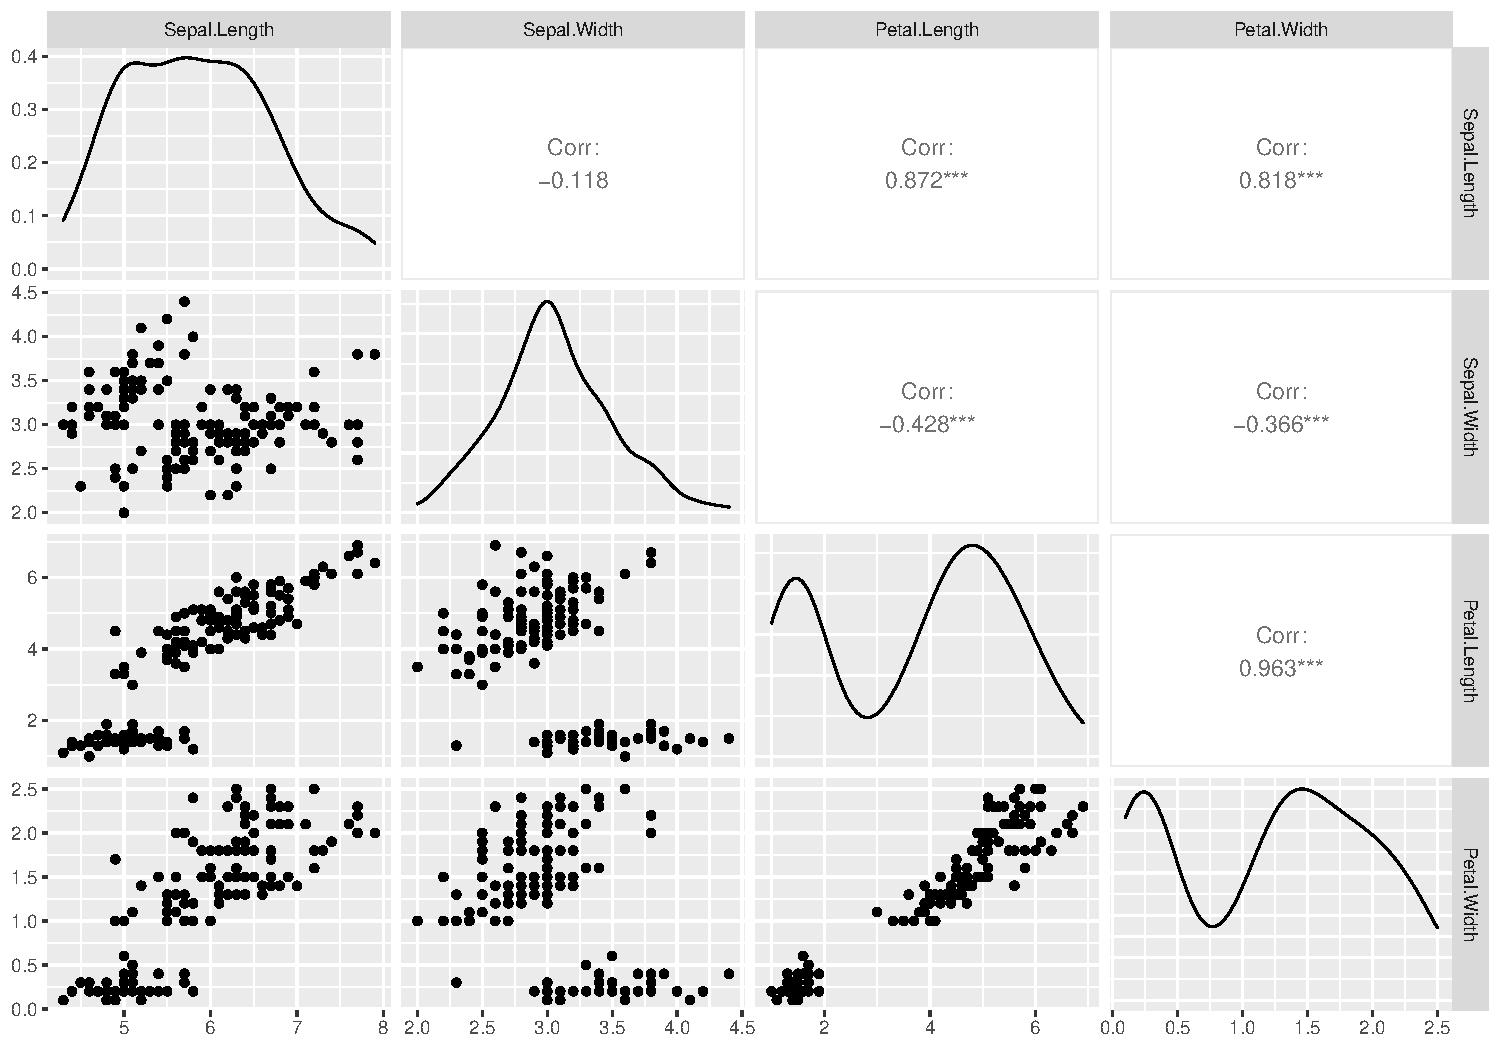
\includegraphics[width=0.7\linewidth,height=0.6\textheight]{figs/unnamed-chunk-1} \end{center}

\normalsize

\end{frame}

\begin{frame}[fragile]{Using PCR}
\protect\hypertarget{using-pcr}{}

\tiny

\begin{Shaded}
\begin{Highlighting}[]
\KeywordTok{library}\NormalTok{(dplyr)}
\KeywordTok{set.seed}\NormalTok{(}\DecValTok{1234}\NormalTok{)}

\CommentTok{# Plotting the feature importance.}
\NormalTok{pcomp_df <-}\StringTok{ }\NormalTok{iris }\OperatorTok\StringTok{ }
\StringTok{  }\KeywordTok{select}\NormalTok{(}\OperatorTok{-}\NormalTok{Species) }\OperatorTok\StringTok{ }\KeywordTok{prcomp}\NormalTok{(}\DataTypeTok{scale. =}\NormalTok{ T, }\DataTypeTok{center =}\NormalTok{ T) }\OperatorTok
\StringTok{  }\KeywordTok{plot}\NormalTok{(}\DataTypeTok{type=}\StringTok{"l"}\NormalTok{, }\DataTypeTok{main =} \StringTok{"Principle Components"}\NormalTok{)}
\end{Highlighting}
\end{Shaded}

\begin{center}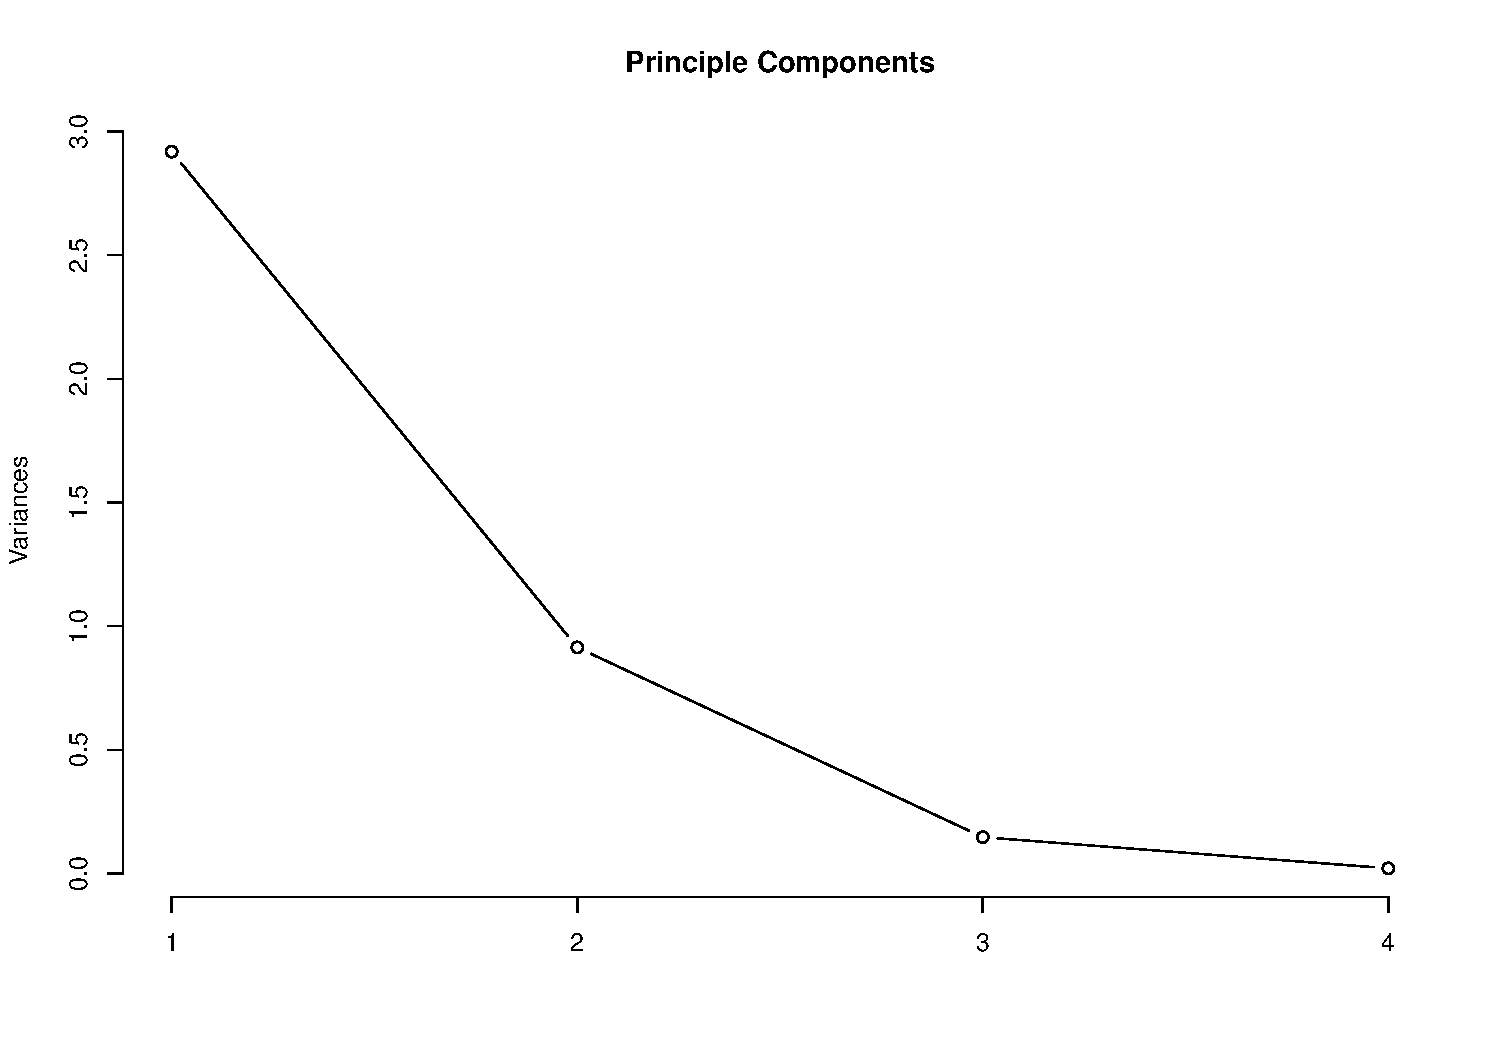
\includegraphics[width=0.7\linewidth,height=0.6\textheight]{figs/unnamed-chunk-2} \end{center}

\normalsize

\end{frame}

\begin{frame}[fragile]{Example of \texttt{\{Boruta\}}}
\protect\hypertarget{example-of-1}{}

\tiny

\begin{Shaded}
\begin{Highlighting}[]
\KeywordTok{library}\NormalTok{(Boruta)}
\KeywordTok{set.seed}\NormalTok{(}\DecValTok{1234}\NormalTok{)}

\CommentTok{# Boruta is a feature selection algorithm based on the random forests algorithm.}
\NormalTok{boruta_df <-}\StringTok{ }\KeywordTok{Boruta}\NormalTok{(Species }\OperatorTok{~}\StringTok{ }\NormalTok{., }\DataTypeTok{data=}\NormalTok{iris, }\DataTypeTok{doTrace=}\DecValTok{0}\NormalTok{)}

\CommentTok{# Plotting the feature importance.}
\KeywordTok{plot}\NormalTok{(boruta_df, }\DataTypeTok{xlab=}\StringTok{"Features"}\NormalTok{, }\DataTypeTok{main=}\StringTok{"Variable Importance"}\NormalTok{)}
\end{Highlighting}
\end{Shaded}

\begin{center}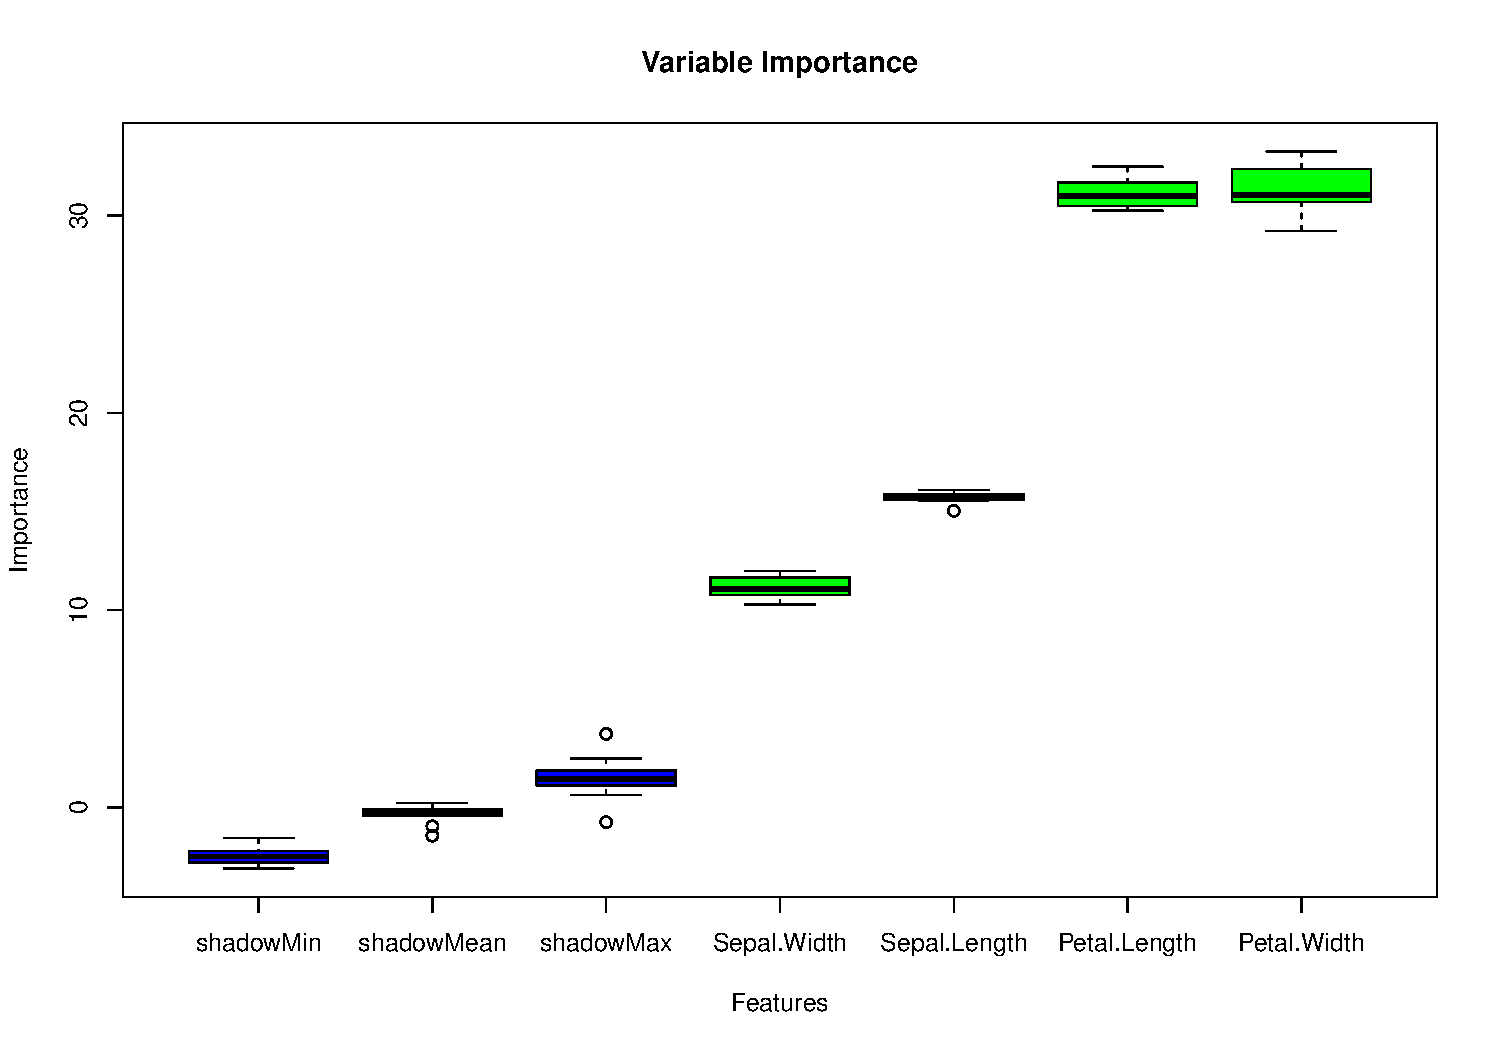
\includegraphics[width=0.7\linewidth,height=0.6\textheight]{figs/unnamed-chunk-3} \end{center}

\normalsize

\end{frame}

\begin{frame}[fragile]{Example of \texttt{\{caret\}}}
\protect\hypertarget{example-of-2}{}

\tiny

\begin{Shaded}
\begin{Highlighting}[]
\KeywordTok{library}\NormalTok{(caret)}
\KeywordTok{set.seed}\NormalTok{(}\DecValTok{1234}\NormalTok{)}

\CommentTok{# Build a decision tree model using rpart (Recursive Partitioning And Regression Trees)}
\NormalTok{rPart_df <-}\StringTok{ }\KeywordTok{train}\NormalTok{(Species }\OperatorTok{~}\StringTok{ }\NormalTok{., }\DataTypeTok{data=}\NormalTok{iris, }\DataTypeTok{method=}\StringTok{"rpart"}\NormalTok{)}
\NormalTok{rPart_imp <-}\StringTok{ }\KeywordTok{varImp}\NormalTok{(rPart_df)}

\CommentTok{# Plotting the feature importance.}
\KeywordTok{plot}\NormalTok{(rPart_imp, }\DataTypeTok{top =} \DecValTok{3}\NormalTok{, }\DataTypeTok{main=}\StringTok{'Variable Importance'}\NormalTok{, }\DataTypeTok{ylab =} \StringTok{"Features"}\NormalTok{)}
\end{Highlighting}
\end{Shaded}

\begin{center}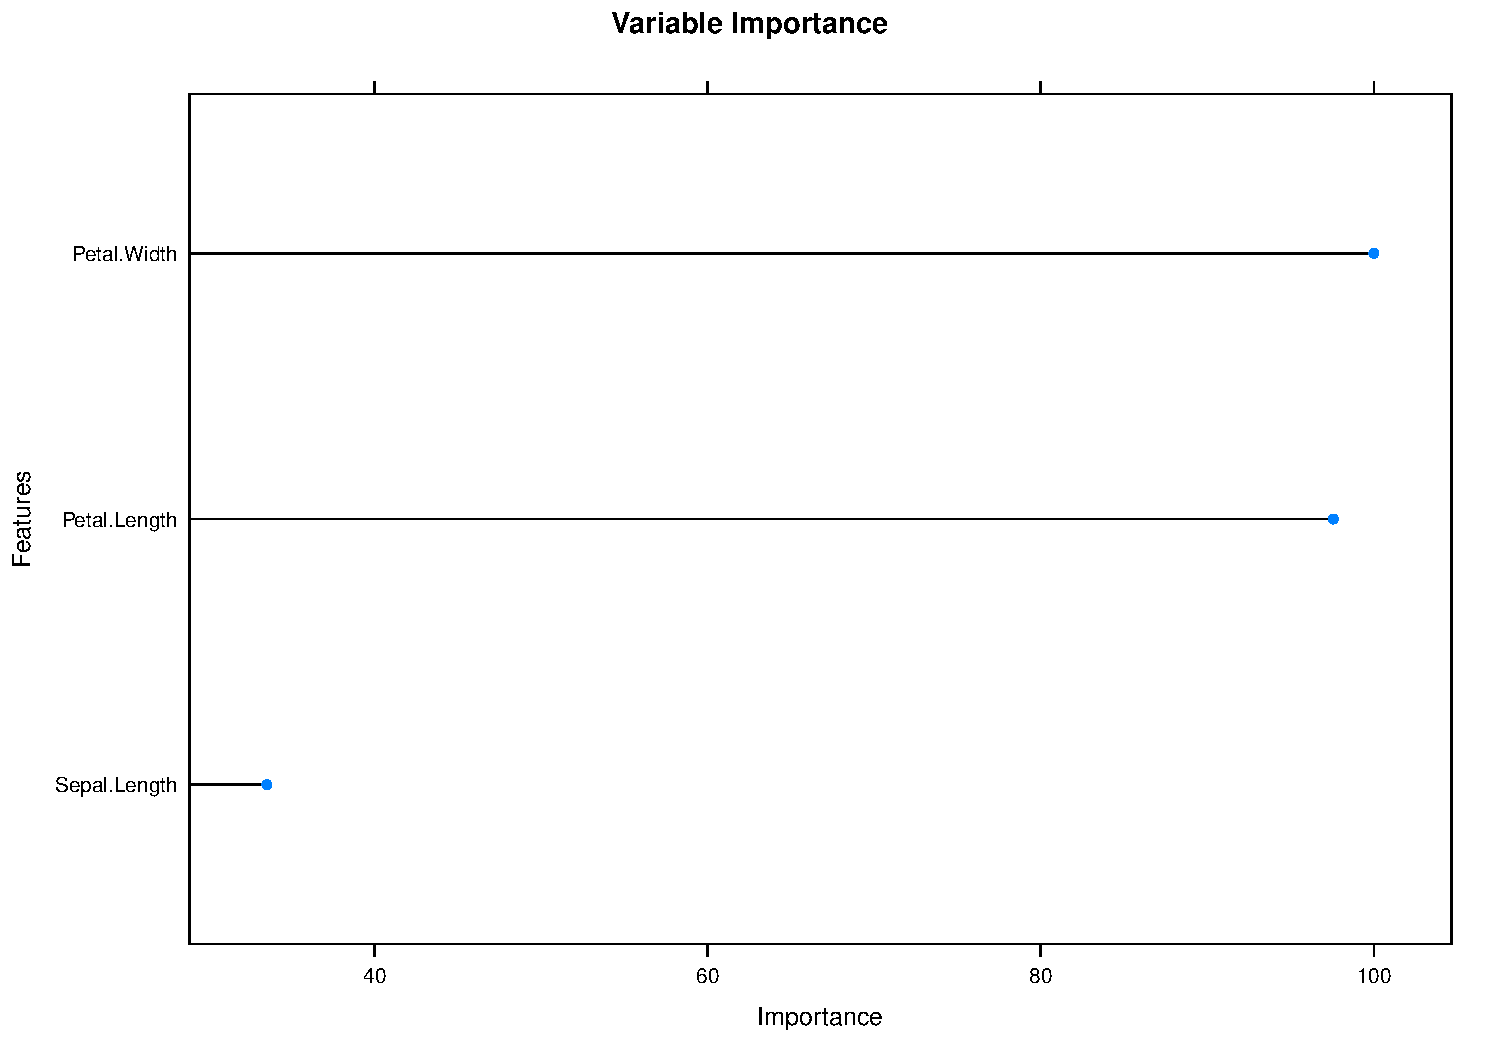
\includegraphics[width=0.7\linewidth,height=0.6\textheight]{figs/unnamed-chunk-4} \end{center}

\normalsize

\end{frame}

\begin{frame}{Explore (E)}
\protect\hypertarget{explore-e}{}

\begin{itemize}
\tightlist
\item
  Examination of data, features, and their characteristics. \vspace{2mm}

  \begin{itemize}
      \item Data types: numerical, ordinal, and nominal data.
      \item Summary statistics.
      \item Feature distributions.
      \item Feature correlations (positive, negative).
      \item Classification: class distribution (\textbf{Class Imbalance?})
  \end{itemize}
   \vspace{2mm}
\item
  Invest your time more on the data exploration process.

  \begin{itemize}
      \item Frequency distribution: \textbf{Histograms}
      \item Outlier detection: \textbf{Box plots}
      \item Feature correlation analysis: \textbf{Scatter plots}
      \item Time series analysis: \textbf{Trend and Seasonal plots}
  \end{itemize}
\end{itemize}

\end{frame}

\begin{frame}{Tools available for Exploration}
\protect\hypertarget{tools-available-for-exploration}{}

\begin{figure}
  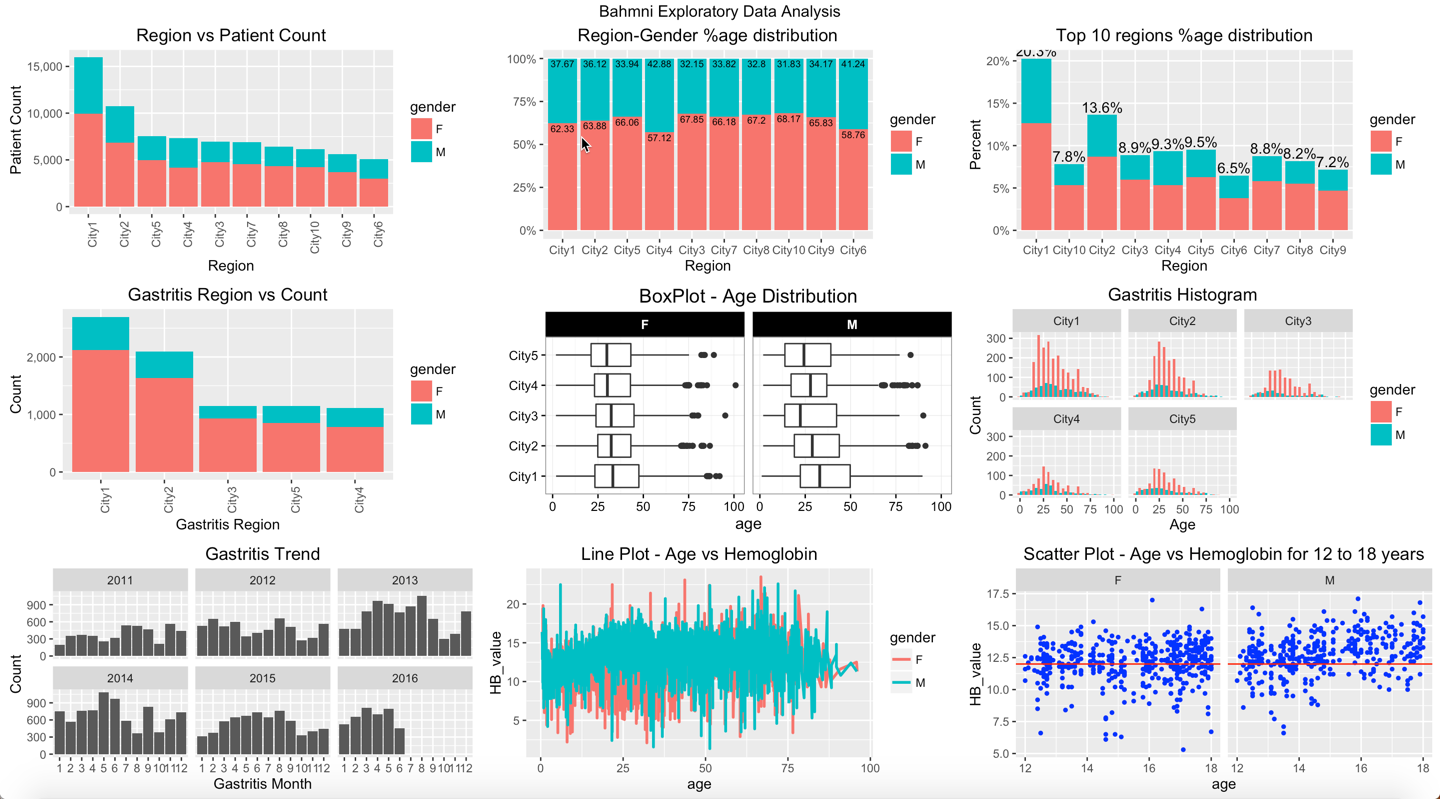
\includegraphics[width=.9\textwidth,height=.9\textheight,keepaspectratio]{images/data_exploration.png}
  \caption{Plots available from \texttt{\{ggplot2\}}%
    \footnote{%
     \tiny{Image source: https://www.pinterest.com.au/pin/281686151677624808/}
    }%
  }
\end{figure}

\end{frame}

\begin{frame}{Seasonal plot from \texttt{\{feasts\}}}
\protect\hypertarget{seasonal-plot-from}{}

\begin{figure}
  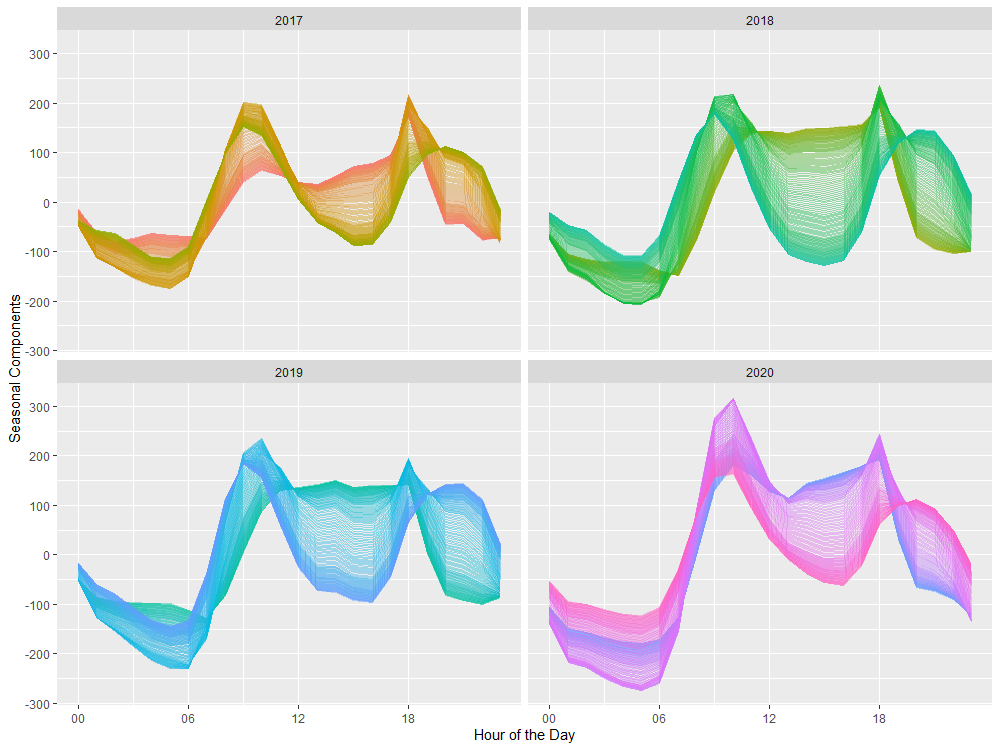
\includegraphics[width=.55\textwidth,height=.55\textheight,keepaspectratio]{images/daily_seasonal.png}
  \caption{The presence of multiple seasonal cycles%
    \footnote{%
     \tiny{Github repo: https://github.com/kasungayan/Meldatathon2020} 
    }%
  }
\end{figure}

\end{frame}

\hypertarget{title-formats}{%
\section{Title formats}\label{title-formats}}

\begin{frame}{Animation (using \LaTeX~)}
\protect\hypertarget{animation-using}{}

\begin{itemize}[<+- | alert@+>]
  \item \alert<4>{This is\only<4>{ really} important}
  \item Now this
  \item And now this
\end{itemize}

\end{frame}

\begin{frame}{Simple list}
\protect\hypertarget{simple-list}{}

\begin{itemize}
  \item Kasun
  \item Now this
  \item And now this
\end{itemize}

\end{frame}

\begin{frame}{Tables (using \LaTeX\})}
\protect\hypertarget{tables-using}{}

\end{frame}

                    \renewcommand\refname{References}
              \begin{frame}[allowframebreaks]{References}
    \bibliographytrue
    \bibliography{references.bib}
    \end{frame}
  


\end{document}
